\section{\label{numerical results}Numerical Results}
\subsection{\label{models}Models}

We considered five models for the population covariance matrix. For the first four settings, $\bs{\Sigma} = \text{diag}(\bs{s}) \bs{C} \text{diag}(\bs{s})$, where $\bs{C}$ is correlation matrix and $\bs{s}$ is a vector of standard deviations.
\begin{itemize}
\item Model 1. The standard deviations were independently generated from $\mathcal{U}(1,1.5)$ and the correlation matrix followed Model 2 of \citet{cai2011adaptive}:
  \[
  \bs{C}=
  \begin{pmatrix}&\bs{A}_1 & \bs{0} \\ &\bs{0} &\bs{I}_{p/2\times p/2}\end{pmatrix},
  \]
  where the $jk$th entry of $\bs{A}_1$ is $a_{jk} = \max(1- \vert j - k \vert / 10, 0)$. This setting modeled a sparse covariance matrix.
  
\item Model 2. The first $p / 2$ standard deviations equaled 1, the last $p / 2$ equaled 2, and the correlation matrix was
  \[
  \bs{C} = \begin{pmatrix} & \bs{C}_{11} & \bs{C}_{12} \\  & \bs{C}_{21} & \bs{C}_{22}\end{pmatrix},
  \]
  where $\bs{C}_{11}$ and $\bs{C}_{22}$ were $p/2 \times p/2$ compound symmetric matrices with correlation parameters 0.8 and 0.2, respectively, and $\bs{C}_{12}$ and $\bs{C}_{21}$ were $p/2 \times p/2$ matrices with entries equal to 0.4. This model was designed such that larger $\sigma_j$ and $\sigma_k$ tended to correspond to larger $r_{jk}$.
  
\item Model 3. The standard deviations were generated independently from $\mathcal{U}(1, 1.5)$ and $\bs{C}$ was a compound symmetric matrix with correlation parameter 0.7. This modeled a dense covariance matrix.
  
\item Model 4. This setting was the same as Model 3 except with correlation parameter 0.9. This high level of dependence tested the robustness of the pairwise composite likelihood estimator \eqref{Gp hat}.
  
\item Model 5. With $\bs{U}$ a randomly generated orthogonal matrix, $\bs{\Sigma} = \bs{U}^T\text{diag}(\bs{l})\bs{U}$, where $\bs{l}$ was a vector of eigenvalues where the first $p / 2$ equaled 1 and the last $p / 2$ equaled 4. This followed simulation settings from \citet{lam2016nonparametric} and \citet{ledoit2019quadratic}.
\end{itemize}

In each scenario, we generated $n=100$ samples from a $p$-variate $\mathcal{N}(\bs{0}, \bs{\Sigma})$, where $p = 30, 100,$ or $200$. We generated $200$ replicates and reported average errors under the following three norms, where $\hat{\bs{\Sigma}}$ is the estimated matrix with entries $\hat{\sigma}_{jk}$ and $\bs{\Sigma}$ is the true matrix with entries $\sigma_{jk}$:
\begin{itemize}
\item Frobenius: $\Vert \hat{\bs{\Sigma}} - \bs{\Sigma} \Vert_F = \{ \sum_{j,k = 1}^p (\hat{\sigma}_{jk} - \sigma_{jk})^2 \}^{1/2}$, a version of \eqref{frobenius risk},
  
\item Spectral: $\Vert \hat{\bs{\Sigma}} - \bs{\Sigma} \Vert_2 = \lambda_{\max}(\hat{\bs{\Sigma}} - \bs{\Sigma})$, the largest eigenvalue of $\hat{\bs{\Sigma}} - \bs{\Sigma}$, and

\item Matrix $\ell_1$: $\Vert \hat{\bs{\Sigma}} - \bs{\Sigma} \Vert_{L_1} = \max_{k = 1, \ldots, p} \sum_{j = 1}^p \vert \hat{\sigma}_{jk} - \sigma_{jk} \vert$.
\end{itemize} 

\subsection{\label{optimalK}Clustering-based exemplar algorithm}
We first studied the behavior of our $K$-means clustering-based exemplar algorithm for different $K$, described in Section \ref{implementation}. For a given $p$, we let $K = rp$ for different ratios ratios $r=2,1,0.5,0.25$. We compared these choices for $K$ to the full exemplar method. For all these estimators, we show the result after applying positive-definiteness correction.

\begin{figure}
  \centering
  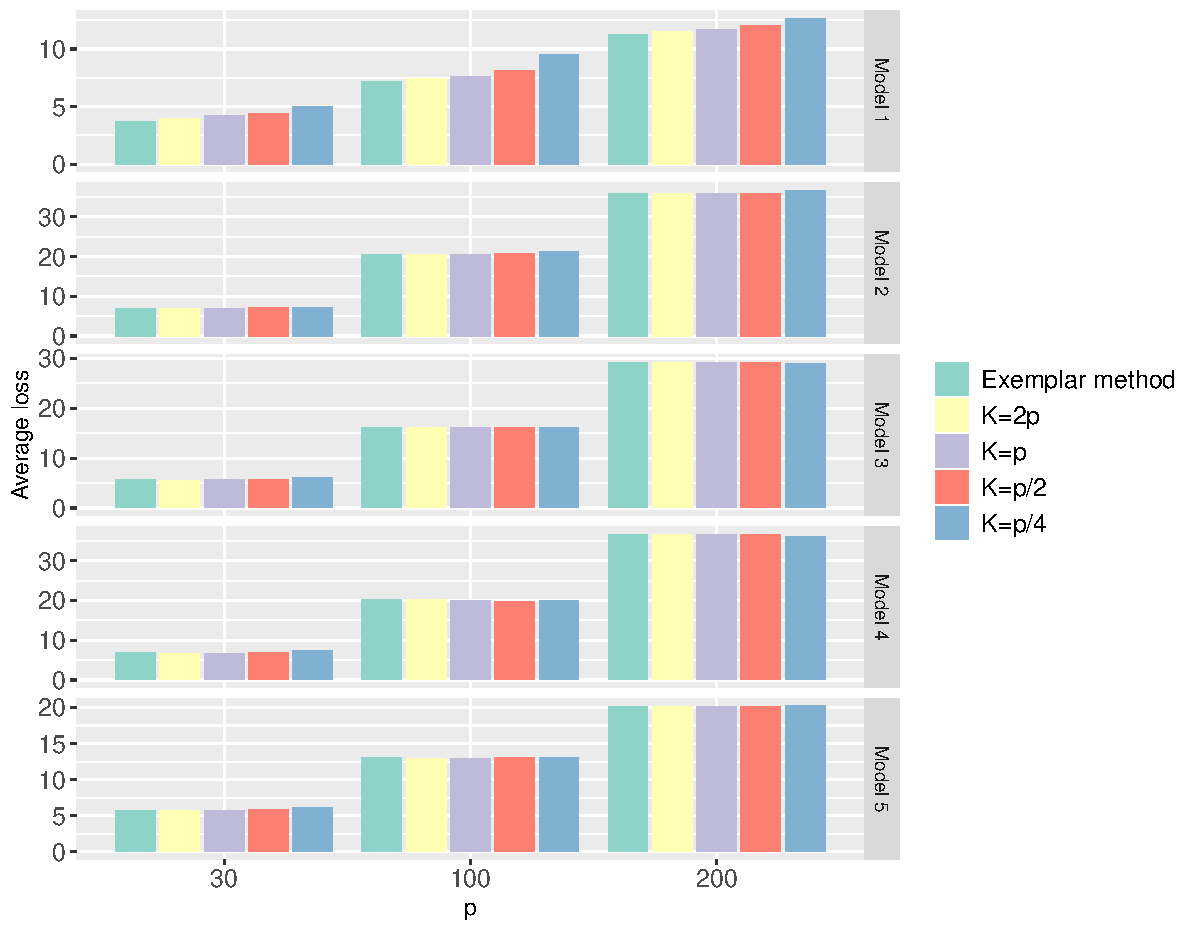
\includegraphics[width=0.85\textwidth]{img/sim1_frobenius.pdf}
  \caption{Average Frobenius norm errors over 200 replications. The Sparse, Block, Dense, Dense2, and Orth panels correspond to Models 1 through 5, respectively.}
  \label{fig:sim1_frobenius}
\end{figure}

\begin{table}
\centering
\setlength{\tabcolsep}{3pt} % Default value: 6pt
\begin{tabular}{rccc}
\hline
            & p=30 & p=100 & p=200 \\
\hline
Exemplar method   & 0.0748          & 4.2575         & 47.8616       \\
$K=2p$	      & 0.0445 	     & 1.3166	   & 12.2612         \\
$K=p$            & 0.0291         & 0.8744         & 8.0862         \\
$K=p/2$         & 0.0207         & 0.5861         & 5.3757         \\
$K=p/4$      & 0.0153         &0.4132          & 3.7415         \\
\hline
\end{tabular}
\caption{\label{tab:sim1_time} Average running time for different ratios.}
\end{table}

Figure \ref{fig:sim1_frobenius} presents the Frobenius norm error estimates from Model 1 to Model 5. Table \ref{tab:sim1_time} shows the running time only for Model 1, because the running time does not vary much across different models. The results show that different $K$ exhibit similar performance and are comparable to the full exemplar method. Letting $K = p$ seemed to provide a good balance between accuracy and speed, so we implement our proposed method with $K = p$ in the rest of this paper.

\subsection{\label{compared}Methods compared}

In this section we refer to our approach using the abbreviation MSG: Matrix Shrinkage via $G$-modeling; we use MSGCor to refer to the version corrected for postive-definiteness. We compared MSG and MSGCor to several existing high-dimensional covariance matrix estimation methods:

\begin{itemize}
\item Sample: the sample covariance matrix.
  
\item Linear: the linear shrinkage estimator of \citet{ledoit2004well} given in \eqref{linear model}.
  
\item QIS: the Quadratic-Inverse Shrinkage estimator of \citet{ledoit2019quadratic}, a recently developed nonlinear shrinkage method. QIS performs linear shrinkage on the sample eigenvalues of the covariance matrix in inverse eigenvalue space. A bandwidth parameter is required, which we choose following the paper's recommendation.
  
\item NERCOME: the Nonparametric Eigenvalue-Regularized COvariance Matrix Estimator of \citet{lam2016nonparametric}. This nonlinear shrinkage method randomly splits the samples into two groups, one for estimating eigenvectors and the other for estimating eigenvalues. Combining the estimates gives a matrix. Following the article, we repeated this procedure 50 times and took the final covariance matrix estimator to be the average of the individual matrices.
  
\item Adap: the adaptive thresholding method of \citep{cai2011adaptive} for sparse covariance matrices, which applies soft thresholding to entries of the sample covariance matrix. The threshold method is adaptive to the entry's variance and involves a tuning parameter. We fixed the parameter at 2, as recommended.
\end{itemize}

In addition to the above estimators, we also implemented the two following oracle estimators, which cannot be implemented in practice as they require the unknown $\bs{\Sigma}$.
\begin{itemize}
\item OracNonlin: the optimal rotation-invariant covariance estimator, defined in \citet{ledoit2019quadratic}, with $\bs{\Sigma} = \bs{U}^T\text{diag}(\bs{l})\bs{U}$, where $\bs{U}=(\bs{u}_1\ldots\bs{u}_p)$ is the sample eigenvector matrix and $\bs{l} = (d_1, \ldots, d_p)$ is composed of oracle eigenvalues $d_i = \bs{u}_i^T\bs{\Sigma} \bs{u}_i$. The sample covariance, the linear shrinkage estimator of \citet{ledoit2004well}, and the nonlinear shrinkage estimators QIS and NERCOME are all rotation-invariant.
  
\item OracMSG: the optimal covariance estimator in the class of separable estimators $\mathcal{S}$ \eqref{separable}. It equals our proposed estimator \eqref{proposed} except with the true $G_p$ \eqref{bayesian} instead of $\hat{G}_p$ \eqref{Gp hat}. The adaptive thresholding method of \citet{cai2011adaptive} also targets a separable estimator.
\end{itemize}

\begin{figure}
  \centering
  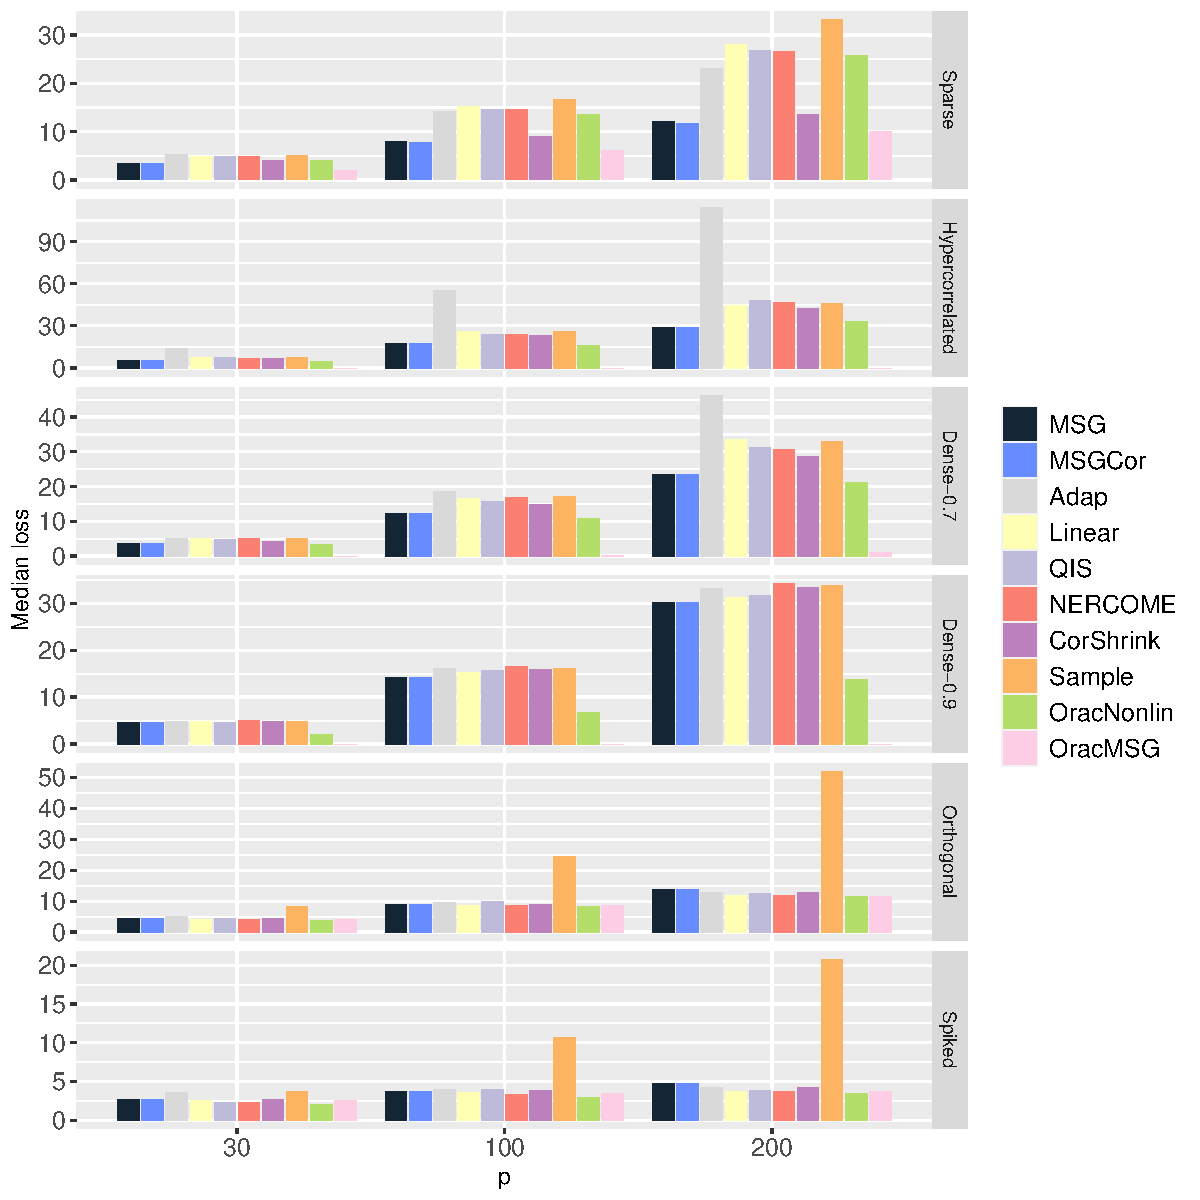
\includegraphics[width=0.85\textwidth]{img/sim2_frobenius.pdf}
  \caption{Average Frobenius norm errors over 200 replications. The Sparse, Block, Dense, Dense2, and Orth panels correspond to Models 1 through 5, respectively.}
  \label{fig:sim2_frobenius}
\end{figure}


Figures \ref{fig:sim2_frobenius} presents the Frobenius loss for different estimators. Our MSG methods had the lowest or near-lowest errors across all settings except for Model 4 which has high correlations 0.9. This is not surprising because our method assumed independence of $\bs{A}_{jk}$.  In some cases, for example in Models 1 and 2, the improvement was substantial. Model 2 was especially interesting because the standard deviation and correlations were related. Our proposed empirical Bayes estimator was able to capture this dependence in its estimate of the prior $G_p$ \eqref{bayesian} and leverage it to provide much more accurate estimates. The nonlinear shrinkage estimators very slightly outperformed MSG in Model 5. In every setting, correcting MSG for positive-definiteness never increased the risk and decreased the risk in some cases. We also did experiments for Spectral norm and Matrix $\ell_1$. The results for this two norms are very similar to Frobenius norm. One exception is Adap has the lowest error in terms of Matrix $\ell_1$ norm in Model 1 because of its sparsity. Though our estimator was motivated in terms of the Frobenius norm error, it performed extremely well in terms of the other two norms as well.

%We were surprised to find that our proposed MSG methods with $d = 30$ did not perform as well as with $d = 20$, and in some cases, especially Model 4, were much worse. Intuitively, more grid points should lead to more accurate results. Indeed, we ran additional simulations using MSG with $d = 5$ and $d = 10$ and found that those results were consistent with this intuition. We believe the counterintuitive performance of $d = 30$ stems from the specific values of the specific points comprising the grid \eqref{grid} in these simulations. In a set of unreported experiments, we let $r_{jk}$ be supported on equally spaced points between the smallest and largest observed sample correlations, instead of between $[-1, 1]$ as in \eqref{grid}. In these results, $d = 20$ and $d = 30$ had similar performance, though neither performed as well as the positive-definite-corrected MSG with $d = 20$ reported here. It was computationally infeasible to implement $d$ much higher than 30. This highlights the importance of developing better computational strategies for multivariate $g$-modeling problems \citep{tao2014convex}.

Finally, the simulations show that the class of separable estimators \eqref{separable} proposed in this paper is fundamentally different from the class of rotation-invariant estimators, as the oracle optimal estimators in these two classes behave very differently. For example, the oracle separable estimator had vanishing risk in Model 2, while the oracle rotiation-invariant estimator does not. Separable estimators seemed better for Models 1 and 2 while rotation-invariant estimators were superior in Models 3 and 4. They seem comparable in Model 5.

\subsection{Data analysis}
\label{gene analysis}
Covariance matrix estimation is often used to reconstruct gene networks \citep{markowetz2007inferring}. We applied our MSG and the other covariance matrix estimators described in Section \ref{compared} to gene network estimation using data from a small round blue-cell tumor microarray experiment, which was also studied by \citet{cai2011adaptive}. \citet{osareh2009classification} report the expression of 2308 genes from 63 samples from four groups: 12 neuroblastoma, 20 rhabdomyosarcoma, 8 Burkitt lymphoma, and 23 Ewing's sarcoma patients. We followed the same data preprocessing as \citet{cai2011adaptive} and sorted the genes in decreasing order according to their $F$-statistic
\begin{equation}
F = \frac{1}{k-1}\sum_{m=1}^kn_m(\bar{x}_m - \bar{x})^2 /   \frac{1}{n-k}\sum_{m=1}^k (n_m-1)\hat{\sigma}_m^2 
\end{equation}
where $k = 4$ is the number of patient categories, $n_m$, $\bar{x}_m$, and $\hat{\sigma}_k$ represent the sample size, sample mean, and sample variance of the gene's expression in the $m$th category, respectively, and $\bar{x}$ is the global mean. We proceeded with the top 40 genes and bottom 160 genes.

We applied various methods to estimate the covariance matrix of these 200 genes. To measure the accuracy of the estimators, we split the 63 samples into two subsets $\bs{X}_1$ and $\bs{X}_2$, ensuring that each subset consisted of the same number of subjects from each of the four disease groups. After centering the variables to have zero mean, we used $\bs{X}_1$ to calculate covariance matrix estimates and compared these to the sample covariance matrix $\bs{S}_2$ of $\bs{X}_2$, which served as a proxy for the unknown true covariance matrix. We measured the errors using the Frobenius, spectral, and matrix $\ell_1$ norms. We repeated this process 200 times.

Table \ref{tab:tab1} reports the average errors across the replications. Our MSG methods had the lowest average error. The positive-definiteness correction slightly reduced the risk as well. The linear shrinkage estimate was almost as accurate, but the other methods were much less accurate. These results suggest that our estimator can perform well in realistic settings, where the mean-zero multivariate normal distributional assumption on the data may not be met.


\begin{table}
\centering
\setlength{\tabcolsep}{3pt} % Default value: 6pt
\begin{tabular}{rccc}
\hline
            & Frobenius & Spectral & Matrix $\ell_1$ \\
\hline
MSG   & 24.07          & 12.89         & 47.12         \\
MSGCor & \textbf{23.90} & \textbf{12.87}& \textbf{46.63}         \\
Adap        & 28.81          & 17.20         & 50.71         \\
Linear      & 24.59         & 13.57         & 51.43         \\
QIS         & 28.66          & 15.94         & 59.30         \\
NERCOME     & 29.76          & 20.13         & 57.30         \\
Sample      & 28.39          & 16.10         & 57.90         \\
\hline
\end{tabular}
\caption{\label{tab:tab1} Average gene expression covariance matrix estimation errors. Bold entries highlight the smallest errors in each column.}
\end{table}

In addition to comparing the numerical accuracies, we also investigated whether our estimator gave qualitatively different gene networks compared to the other approaches. First, Figure \ref{network} illustrates the covariance matrices in network form, where each node represents a gene and each edge represents a non-zero covariance between the genes it connects. To avoid completely connected graphs, we sparsified the matrix estimates by thresholding the smaller entries of each matrix to zero. Since the adaptive thresholding method of \citet{cai2011adaptive} naturally produced a sparse estimated matrix, we thresholded the other matrix estimates to match the sparsity level of the \citet{cai2011adaptive} estimate.

\begin{figure}
  \centering
  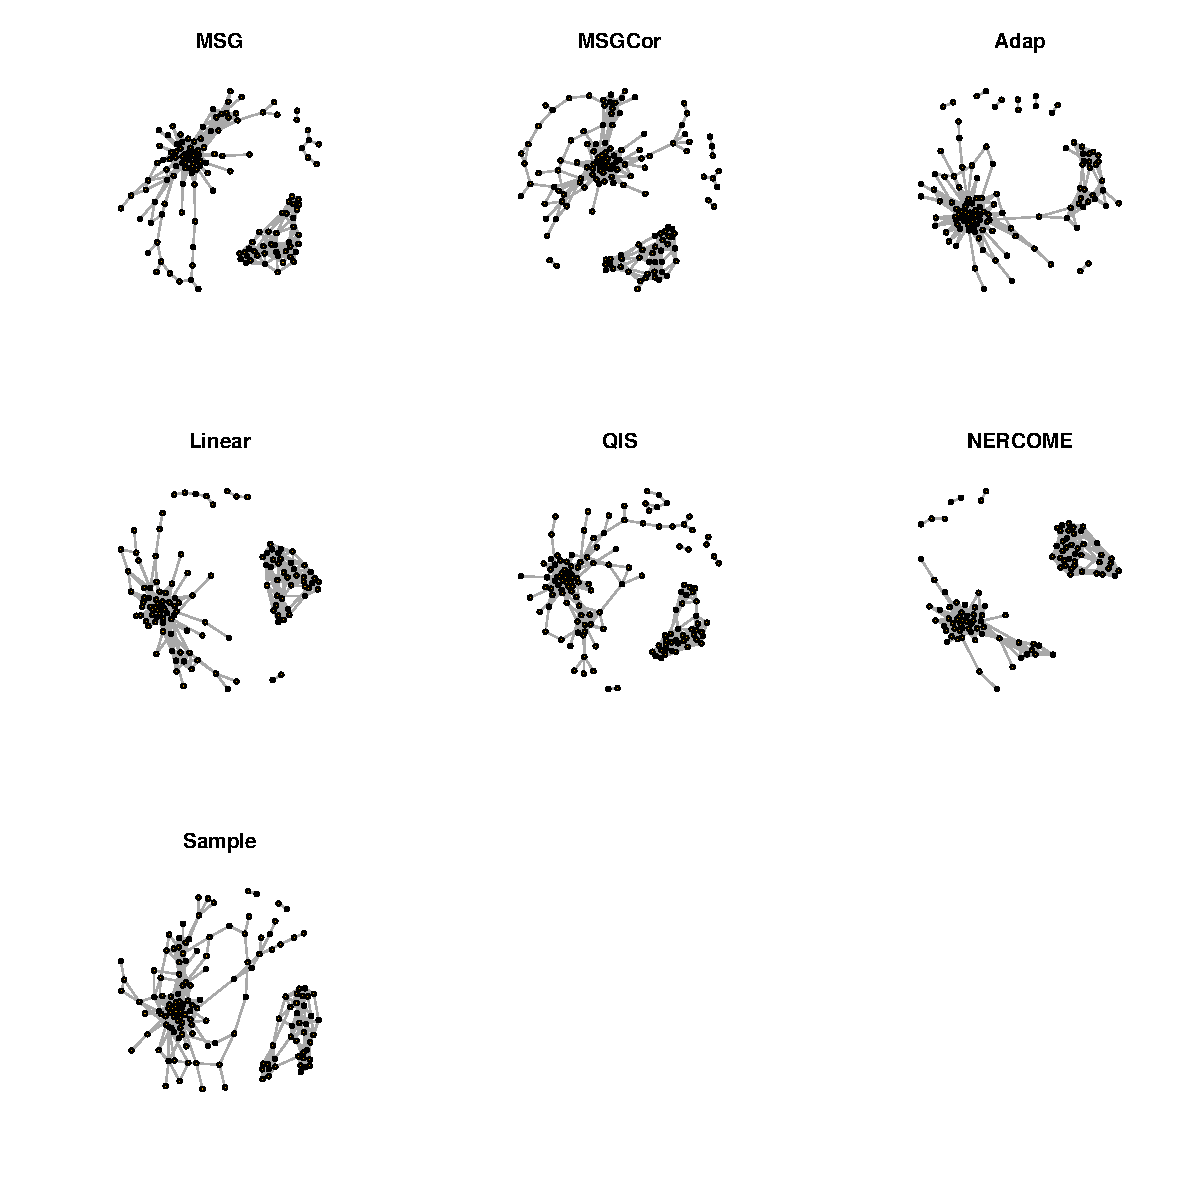
\includegraphics[width=0.85\textwidth]{img/network.pdf}
  \caption{Gene networks recovered by the different covariance matrix estimation methods.}
  \label{network}
\end{figure}

The results show several interesting features. First, there appear to be two major clusters, which are disconnected in every estimated network except for the one produced by the adaptive thresholding approach. Second, the larger cluster appears to contain two sub-clusters, and this finer structure was only recovered by MSG and QIS, and to a lesser extent the linear shrinkage estimator and NERCOME. Finally, the nodes in the networks estimated by QIS and NERCOME appear to be clustered more tightly together compared to in the other networks. These observations suggest that MSG produces qualitatively different networks, in addition to lower estimation errors.

Finally, we also compared the estimated degrees of the genes in the different networks. For each estimated network, we ordered the 200 genes by degree and then selected the top 20\%, denoting this set $J_k$ for the $k$th network. For each pair of networks $k$ and $k'$, we calculated the similarity between their most connected genes using Jaccard index $\vert J_k \cap J_{k'} \vert / \vert J_k \cup J_{k'} \vert$. Figure \ref{top20} visualizes these similarities. Interestingly, however, among all estimators, they were also the most similar to the unbiased sample covariance matrix. Together with the above results, this indicates that MSG may simultaneously give the lowest error and, at least in terms of degree estimation, the most unbiased results.

\begin{figure}
  \centering
  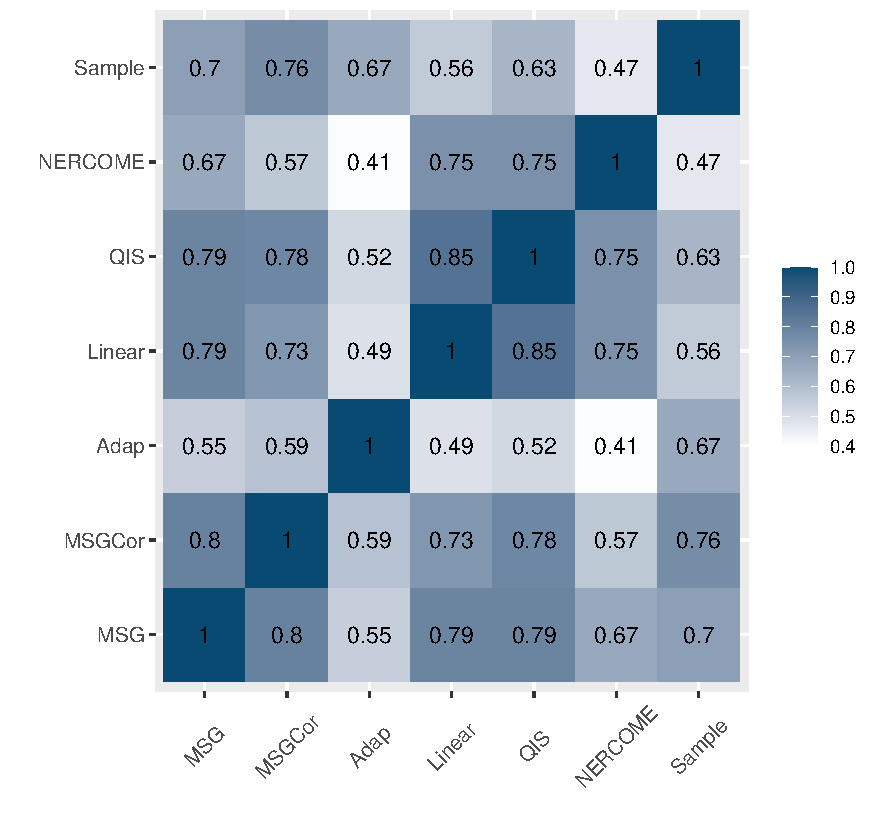
\includegraphics[width=0.85\textwidth]{img/top20.pdf}
  \caption{Similarities of gene degrees between the estimated networks. Each number reports the Jaccard index between the top 20\% most connected genes of each pair of networks.}
  \label{top20}
\end{figure}

%%% Local Variables:
%%% mode: latex
%%% TeX-master: "msg"
%%% End:
